% Erzeugt von Marc Weidner
%
%%%% Documenten Klasse
\documentclass[12pt,oneside,openright]{book}
%%%% Definitionen und Klassen
 % hier wird das Aussehen des Dokumentes definiert und die Pakete die geladen werden. Allegmeine Definitons Gunrdlage für das Design des Dokuments


\usepackage{iftex} % Überprüft, ob das Dokument mit PDFLaTeX, XeLaTeX oder LuaLaTeX kompiliert wird.
\ifPDFTeX
\usepackage[utf8]{inputenc} % Ermöglicht die Eingabe von Umlauten und anderen Sonderzeichen in UTF-8-Kodierung.
\usepackage[T1]{fontenc} % Verbessert die Darstellung von Umlauten und anderen Sonderzeichen in PDF-Dokumenten.
\fi	
\usepackage{lmodern} % Lädt die "Latin Modern" Schriftarten, eine verbesserte Version der Computer Modern Schriftarten.
\usepackage[export]{adjustbox} % Ermöglicht erweiterte Grafikeinstellungen, wie Skalierung, Beschnitt und Rahmen.
\usepackage{graphicx} % Ermöglicht das Einbinden von Grafiken und Bildern.
\usepackage[dvipsnames]{xcolor} % Ermöglicht die Verwendung einer großen Palette von Farben.
\usepackage{url} % Ermöglicht die korrekte Formatierung und Hervorhebung von URLs.
\urlstyle{same} % Setzt den Stil für URLs, sodass sie in derselben Schriftart wie der umgebende Text erscheinen.
\usepackage[sfdefault]{ClearSans} % Lädt die "Clear Sans" Schriftart als Standardsans-Serif-Schriftart.
\usepackage{tabularx} % Ermöglicht erweiterte Tabellenfunktionen, wie automatische Breitenanpassung.
\usepackage{colortbl} % Ermöglicht das Hinzufügen von Farbe zu Tabellenzellen.
\usepackage{textcomp} % Ermöglicht den Zugriff auf Textsymbole.
\usepackage{longtable} % Ermöglicht die Erstellung von Tabellen, die sich über mehrere Seiten erstrecken können.
\usepackage{bmpsize} % Ermöglicht die korrekte Größenbestimmung von Bitmap-Grafiken.
\usepackage{calc} % Ermöglicht die Verwendung von arithmetischen Operationen in LaTeX-Befehlen.
\usepackage{array} % Erweitert die Funktionen und Optionen für Tabellen.
\usepackage{enumitem,amssymb} % `enumitem` ermöglicht individuelle Anpassungen von Listen, `amssymb` lädt zusätzliche mathematische Symbole.
\usepackage[printonlyused,withpage]{acronym} % Ermöglicht die Verwendung von Abkürzungen, wobei nur verwendete Abkürzungen gedruckt und mit Seitenzahlen versehen werden.
%\usepackage[colorlinks]{hyperref} % Ermöglicht das Erstellen von Hyperlinks und PDF-Bookmarks; auskommentiert.
\usepackage[ngerman]{babel} % Stellt sicher, dass das Dokument deutsche Sprachkonventionen verwendet.
\usepackage{float} % Verbessert die Platzierung von Float-Objekten (wie Tabellen und Abbildungen).
\usepackage{hyperref} % Ermöglicht das Erstellen von Hyperlinks und PDF-Bookmarks.
\usepackage{pdfpages} % Ermöglicht das Einbinden von kompletten oder Teilen von PDF-Seiten.
\usepackage{media9} % Ermöglicht das Einbinden von Multimedia-Inhalten (Audio, Video) in PDFs.
\usepackage[bottom=3cm]{geometry} % Einstellung des Seitenlayouts, hier speziell Anpassung des unteren Randes.
\usepackage[headsepline, footsepline]{scrlayer-scrpage} % Laden Sie das scrpage2-Paket für scrheadings




%------------------------------------------------
%  Hinweise
%------------------------------------------------
% Für Pfade kann entweder \path oder \url verwendet werden





%------------------------------------------------
%  Kopf uns Fusszeile
%------------------------------------------------
\ihead{Test Management} % Left header: Document name
\ofoot{\pagemark} % Right footer: Page number
\cfoot{© 2022-2024 PLMBakery } % Clear center footer
\ifoot{\url{http://plmbakery.de}} % Left footer: Website
\setkomafont{pagefoot}{\normalfont} % Font style for footer
\setkomafont{pagehead}{\normalfont\bfseries} % Font style for header
%------------------------------------------------
%  Fusszeile Anpassung wenn Plain verwendet wird wie in den Verzeichnissen am Ende, das mache ich weil dort den Header nicht haben will sondern nur die Fusszeile
%------------------------------------------------





%------------------------------------------------
%  Definiton der Tabellenform für die Texte Bild Links Text Rechts
%------------------------------------------------
\newenvironment{eintrag}[1]{
	\par\medskip\noindent%
	\begin{minipage}[t]{\dimexpr.5\linewidth-10\tabcolsep\relax}
		\strut\\[-\baselineskip]#1
	\end{minipage}\hspace{2\tabcolsep}\begin{minipage}[t]{\dimexpr0.4\linewidth-\tabcolsep\relax}}{\end{minipage}}


%------------------------------------------------
%  Für Screenshots mit 7cm breite und text daneben / verwende ich als Standard nun
%------------------------------------------------
\newenvironment{eintrag2}[1]{
	\par\medskip\noindent%
	\begin{minipage}[t]{\dimexpr.5\linewidth-\tabcolsep\relax}
		\strut\\[-\baselineskip]#1
	\end{minipage}\hspace{1\tabcolsep}\begin{minipage}[t]{\dimexpr.5\linewidth-\tabcolsep\relax}}{\end{minipage}}

%------------------------------------------------
%%% FAQ Idee
%------------------------------------------------
\newcommand{\faqu}[2]{%
	{\textbf{Frage:}} \normalfont\sffamily\textsf{#1}\par
	\noindent{\textbf{\textit{Antwort:}}} #2
}
\newcommand{\sol}[2]{%
	\noindent\rule[1ex]{\textwidth}{0.5pt}
	{\textbf{\textcolor{red}{Issue}}} \normalfont\sffamily\textsf{#1}\par
	\noindent{\textbf{\textcolor{green}{Solution:}}} #2\\
	\noindent\rule[1ex]{\textwidth}{0.5pt}
}

\newcommand{\faq}[2]{%
	\noindent\rule[1ex]{\textwidth}{0.5pt}
	{\textbf{\textcolor{red}{Frage}}} \normalfont\sffamily\textsf{#1}\par
	\noindent{\textbf{\textcolor{green}{Antwort:}}} #2\\
	\noindent\rule[1ex]{\textwidth}{0.5pt}
}

%------------------------------------------------
%  Zuer Erstellung einer Todoliste
%------------------------------------------------
\newlist{todolist}{itemize}{2}
\setlist[todolist]{label=$\square$}







%%%% Titel
\title{KDP Buch Vorlage\\}
\author{Marc Weidner}
%%%% Beginn Dokument
\begin{document}
	\maketitle
	\newpage
	\tableofcontents
	\newpage
	\begin{center}
		\textbf{Copyright © 2023 Marc Weidner}
	\end{center}
		\begin{flushleft}
		Alle Rechte vorbehalten. Dieses Buch und sein gesamter Inhalt sind urheberrechtlich geschützt. Jegliche Vervielfältigung, Verbreitung oder Nutzung, auch auszugsweise, ohne ausdrückliche schriftliche Genehmigung des Autors oder Rechteinhabers ist untersagt.Das Urheberrecht umfasst alle Texte, Bilder, Grafiken, Illustrationen, Tabellen und sonstige Inhalte dieses Buches. Jede unerlaubte Verwendung, Reproduktion oder Verbreitung wird zivil- und strafrechtlich verfolgt. Das Urheberrecht schützt die Ideen und kreativen Ausdrucksformen des Autors. Alle Inhalte dieses Buches sind geistiges Eigentum des Autors und unterliegen dem internationalen Urheberrechtsgesetz.
	\newline
		Die Inhalte dieses Buches dienen ausschließlich Informationszwecken und stellen keine Rechts-, Finanz- oder sonstige professionelle Beratung dar. Der Autor übernimmt keine Haftung für etwaige Schäden oder Verluste, die durch die Verwendung der in diesem Buch enthaltenen Informationen entstehen könnten. Jegliche Verwendung oder Zitierung von Inhalten dieses Buches muss mit entsprechender Quellenangabe erfolgen.
	\newline
		Das Copyright gilt sowohl für die gedruckte als auch für die elektronische Version dieses Buches. Bei Fragen zum Urheberrecht oder zur Nutzung von Inhalten dieses Buches wenden Sie sich bitte an den Autor oder den Rechteinhaber.
	\newline
		Vielen Dank für Ihr Verständnis und Ihre Einhaltung des Urheberrechts.
	\end{flushleft}
	\newpage
	\begin{center}
		\textbf{Danksagung}
	\end{center}
	\lipsum[1-5]
	\begin{figure}[h]
		\centering
		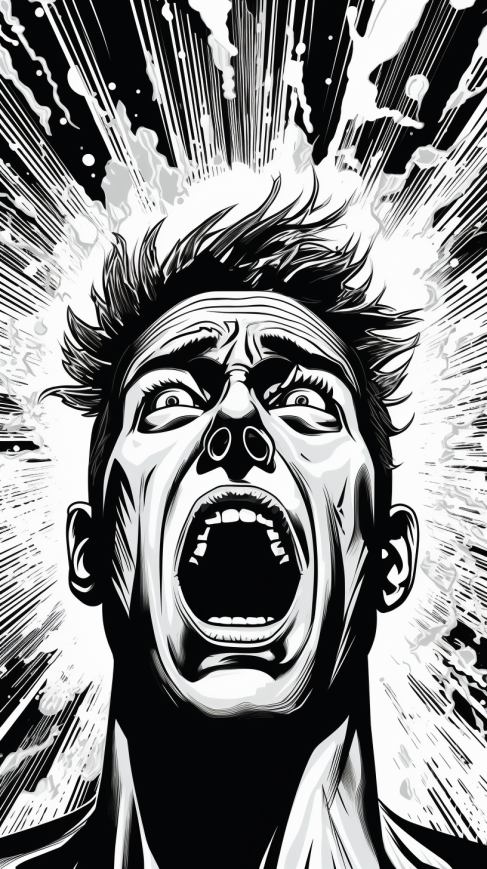
\includegraphics[frame,width=0.5\linewidth]{pics/01}
		\caption[Emotionaler Mensch]{Emotionaler Mensch}
		\label{Emotionaler Mensch}
	\end{figure}
	\newpage
%%%% Kapitel Listing
	\newpage
\thispagestyle{empty}
\quad  \addtocounter{page}{-1}
\newpage
\chapter{Überschrift 1}
\lipsum[1-5]


\chapter*{Schlusswort}
\addcontentsline{toc}{chapter}{Schlusswort}
In diesem Buch sind wir zusammen auf eine Reise gegangen, um die Kunst der Gelassenheit zu erforschen. Von den grundlegenden Prinzipien der Achtsamkeit bis hin zur progressiven Muskelentspannung nach Jacobson, von Entscheidungsstrategien bis zum bewussten Umgang mit digitalen Medien haben wir eine Vielzahl an Themen beleuchtet, die uns dabei helfen können, ein ausgeglicheneres und gelasseneres Leben zu führen.\\
\\
Die Werkzeuge und Übungen, die ich vorgestellt habe, dienen als Leitfaden, um eine neue Balance in unserem hektischen Alltag zu finden. Es ist wichtig zu betonen, dass Veränderung nicht über Nacht geschieht. Es ist ein Prozess, der Geduld, Engagement und die Bereitschaft erfordert, kontinuierlich an sich selbst zu arbeiten.\\
\\
In einer Welt, die sich immer schneller dreht, in der wir ständig erreichbar sind und immer mehr Informationen in kürzerer Zeit verarbeiten müssen, ist es wichtiger denn je, sich bewusst Zeiten der Ruhe und des Innehaltens zu schaffen. Achtsamkeit, Gelassenheit und Entspannung sind keine luxuriösen Extras, sondern grundlegende Bedürfnisse, die uns dabei helfen, gesund und ausgeglichen zu bleiben.\\
\\
Ich hoffe, dass die Inhalte dieses Buches dich dazu inspiriert haben, dir diese Momente der Ruhe bewusst zu schaffen und dich darin unterstützen, neue Wege zu mehr Gelassenheit in deinem Leben zu finden. Denke immer daran: Gelassenheit ist kein Zustand, den man einmal erreicht und dann für immer behält. Es ist eine Fähigkeit, die wir ständig üben und weiterentwickeln können.\\
\\
Zum Abschluss möchte ich dich ermutigen, die hier vorgestellten Übungen und Praktiken auszuprobieren, sie in deinen Alltag zu integrieren und zu beobachten, wie sie sich auf dein Wohlbefinden auswirken. Sei geduldig mit dir selbst, erkenne deine Fortschritte an und feiere sie. Und vor allem, sei achtsam und freundlich zu dir selbst auf dieser Reise.\\
\\
Ich wünsche dir viel Erfolg, Gelassenheit und innere Ruhe auf deinem Weg.
\newpage
\listoffigures

\end{document}